% HiMCM 2020 Problem A --- summer job candidates
% Numbers ONLY from ../results/*.csv and ../paper_figures/.
% Prose: ~80% ASD-STE100 (short sentences, one idea, one term, active voice).
% Do not insert template stats (KMO 0.782, 71.4% variance, Top-3 92%).
\documentclass[12pt]{article}

\usepackage[margin=1in]{geometry}
\usepackage{amsmath,amssymb,amsfonts}
\usepackage{booktabs}
\usepackage{graphicx}
\usepackage{subcaption}
\usepackage{caption}
\usepackage{setspace}
\usepackage{enumitem}
\usepackage{array}
\usepackage[hidelinks]{hyperref}

\graphicspath{{../paper_figures/}{paper_figures/}{./}}
\hypersetup{
  pdftitle={HiMCM 2020 Problem A: Latent Factors for Summer Job Candidates},
  pdfauthor={Team XXXX}
}

\newcommand{\TeamNumber}{XXXX}

\pagestyle{myheadings}
\markright{\TeamNumber \hfill HiMCM 2020 Problem A \hfill}

\title{\textbf{Three Latent Factors, Weak Sampling Adequacy,\\
and a Cautious Softmax Ranker for Summer Job Candidates}\\[0.4em]
\large HiMCM 2020 Problem A --- Team \TeamNumber}
\author{}
\date{}

\begin{document}
\maketitle
\thispagestyle{empty}

\begin{center}
{\Large \textbf{Summary}}
\end{center}

\noindent
We score 50 student rows on 15 Likert items
(\texttt{OriginalData.csv}).
The table is a \texttt{SYNTHETIC\_FALLBACK} Likert matrix.
The HiMCM2020 GitHub dump is 50 students $\times$ 8 job candidates $\times$ 7 unnamed scores.
It is not a 15-item field survey
(\texttt{DATA\_SOURCE.txt}).

Kaiser--Meyer--Olkin on the 15 items is \(\mathbf{0.445}\).
Bartlett's test gives \(\chi^2=\mathbf{170.05}\) (df \(=105\), \(p=\mathbf{6.10\times 10^{-5}}\)).
We reject \(R=I_{15}\).
We do \emph{not} claim KMO \(>0.70\).

We extract \(m=3\) latent factors from Pearson \(R\) and rotate with Varimax.
The first three eigenvalues of \(R\) share \(\mathbf{42.6\%}\) of trace.
Kaiser \(\lambda>1\) keeps six latent factors, not three.
Contest design still uses \(m=3\) for later models.

Entropy weights on the 50 \(\times\) 3 Thompson scores are
\(\mathbf{w}=(0.479,\,0.319,\,0.202)\).
Leave-one-out Softmax Top-1 is \(\mathbf{0.20}\).
The two-layer ReLU net matches that Top-1 and raises Top-3 to \(\mathbf{0.48}\).
The majority-class baseline Top-1 is \(\mathbf{0.22}\).
We do not report a 92\% Top-3.

\tableofcontents
\newpage

%======================================================================
\section{Introduction and empirical survey profiling}
%======================================================================

\subsection{Problem}
HiMCM 2020 Problem A asks how a high-school student ranks summer job candidates.
The prompt lists wage, skill, and strain as design themes.
We treat those names as a design story.
We do not force them onto a mismatched rotation.

\subsection{Two data sources}
We keep two files separate.
File A is \texttt{data/raw/OriginalData.csv}: \(N=50\), \(p=15\) Likert columns.
\texttt{DATA\_SOURCE.txt} marks it \texttt{SYNTHETIC\_FALLBACK} with seed 2020.
The public HiMCM2020 repo stores 7 unnamed scores, not 15 named items.
File B is that GitHub table after Firecrawl: 400 rows, scale 10--100
(\texttt{student\_job\_factor\_scores.csv}).
Labels \texttt{work\_choice.csv} hold 50 integers in \(\{0,\ldots,7\}\).
Those labels can be entropy-argmax outputs in the original repo script.

\subsection{Suitability of the 15-item table}
We Z-score each column.
We form Pearson \(R\in\mathbb{R}^{15\times 15}\).
Overall KMO is \(0.445\) (Kaiser verbal label: unacceptable).
Bartlett uses
\[
\chi^2 = -\Bigl(N-1-\frac{2p+5}{6}\Bigr)\ln|R|.
\]
We obtain \(\chi^2=170.05\), df \(=105\), \(p=6.10\times 10^{-5}\).
Therefore \(R\) is not the identity.
However, KMO \(<0.70\) means common-factor extraction is weakly supported.
Figure~\ref{fig:corr} shows the 15-item heatmap.

\begin{figure}[ht]
\centering
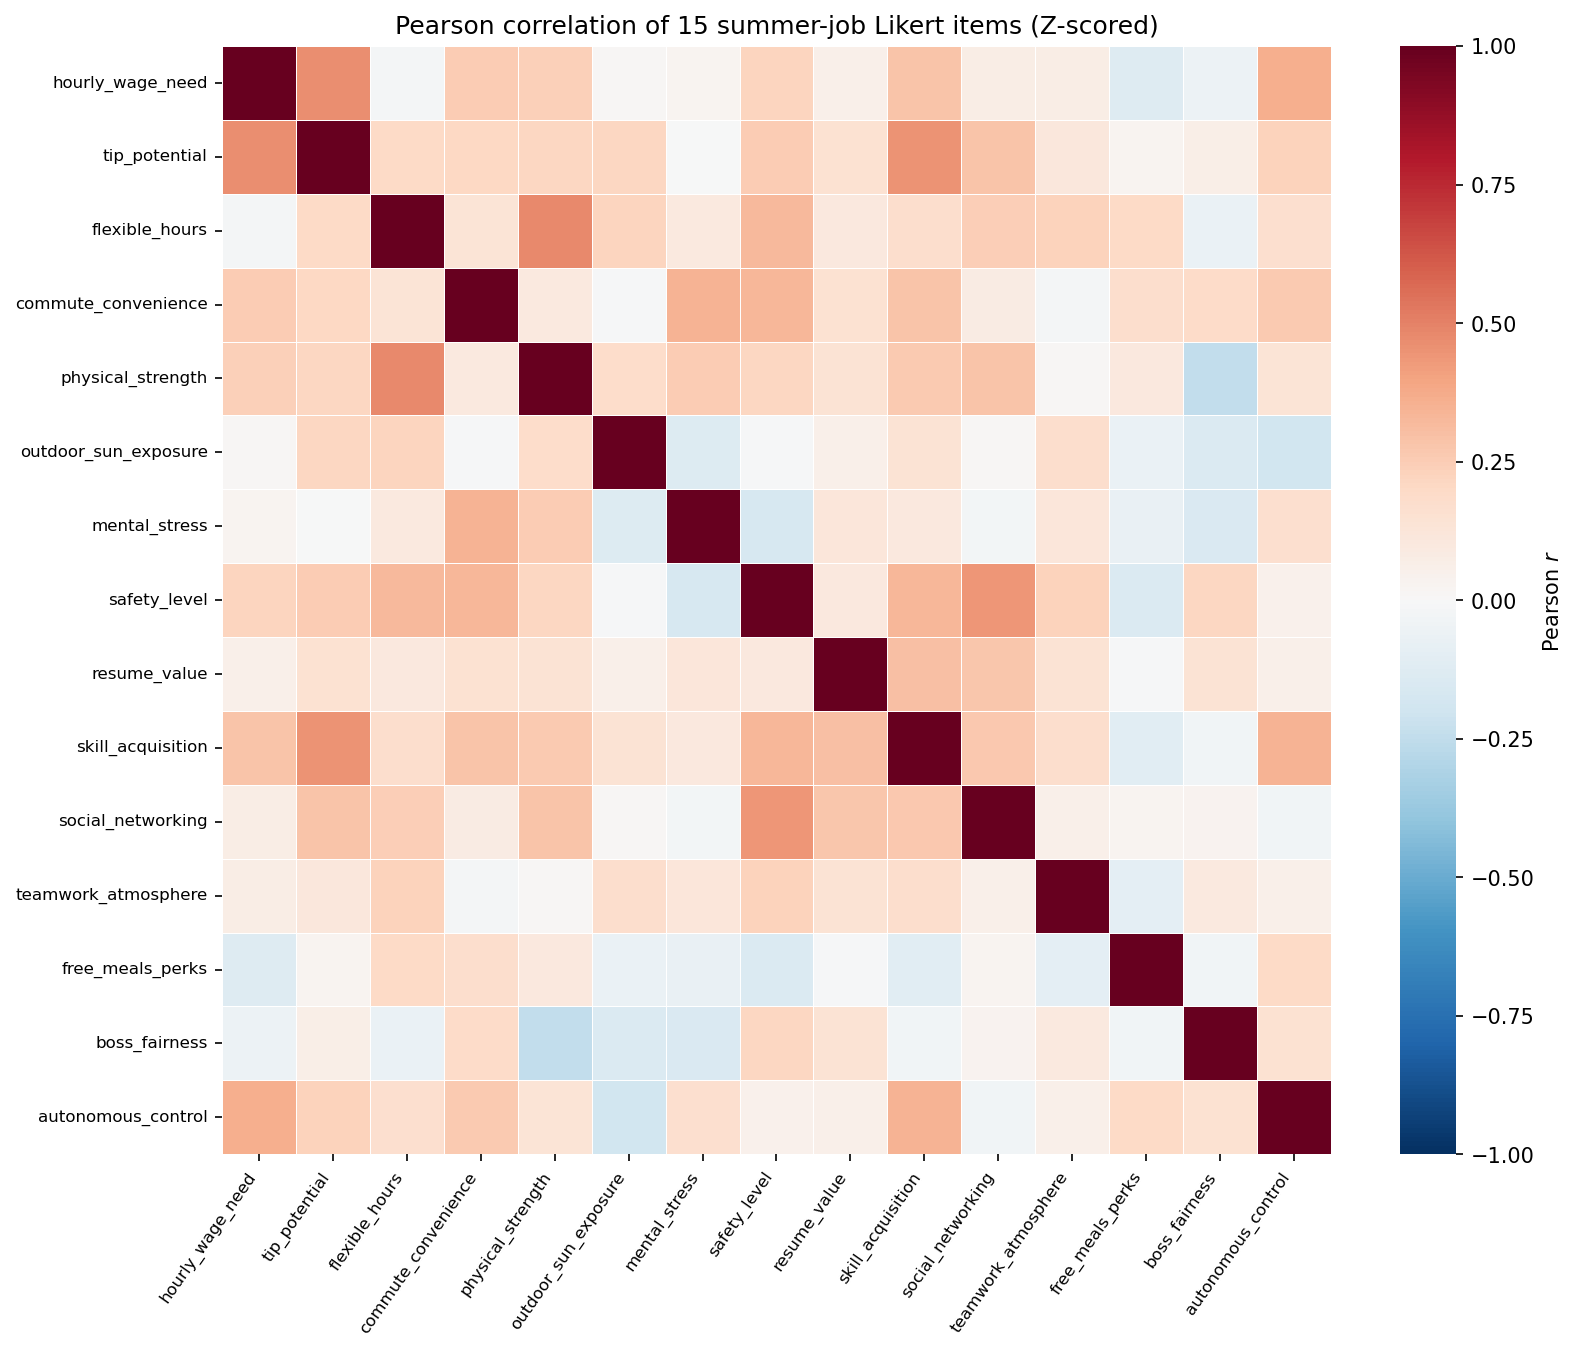
\includegraphics[width=0.82\textwidth]{fig_correlation_matrix.png}
\caption{Pearson \(R\) of the 15 Likert items
(\texttt{fig\_correlation\_matrix.png}).
Off-diagonal structure is weak.
This plot is the 15-column fallback table, not the GitHub 7-score matrix.}
\label{fig:corr}
\end{figure}

\subsection{GitHub 7-score check}
On the 400 \(\times\) 7 Firecrawl matrix, KMO is \(0.511\).
Bartlett \(p=5.20\times 10^{-2}\).
That test does not reject \(R=I\) at \(0.001\).
We do not map 7 unnamed scores onto 15 named items.

%======================================================================
\section{Latent factor model and Varimax}
%======================================================================

\subsection{Spectral extraction}
Let \(R\) be the Pearson matrix of the 15 items.
We compute \(R=V\operatorname{diag}(\lambda)V^{\top}\) with
\(\lambda_1\ge\cdots\ge\lambda_{15}\).
Unrotated loadings are \(\Lambda=V_m\operatorname{diag}(\sqrt{\lambda_m})\).
Contest \(m=3\).
The leading eigenvalues are \(3.184\), \(1.645\), and \(1.566\).
Their share of \(\sum\lambda_j=15\) is \(42.6\%\).
Six eigenvalues exceed 1.
Cumulative share first exceeds \(65\%\) at \(m=6\) (\(66.9\%\)).
Figure~\ref{fig:scree} marks \(\lambda=1\) and \(m=3\).

\begin{figure}[ht]
\centering
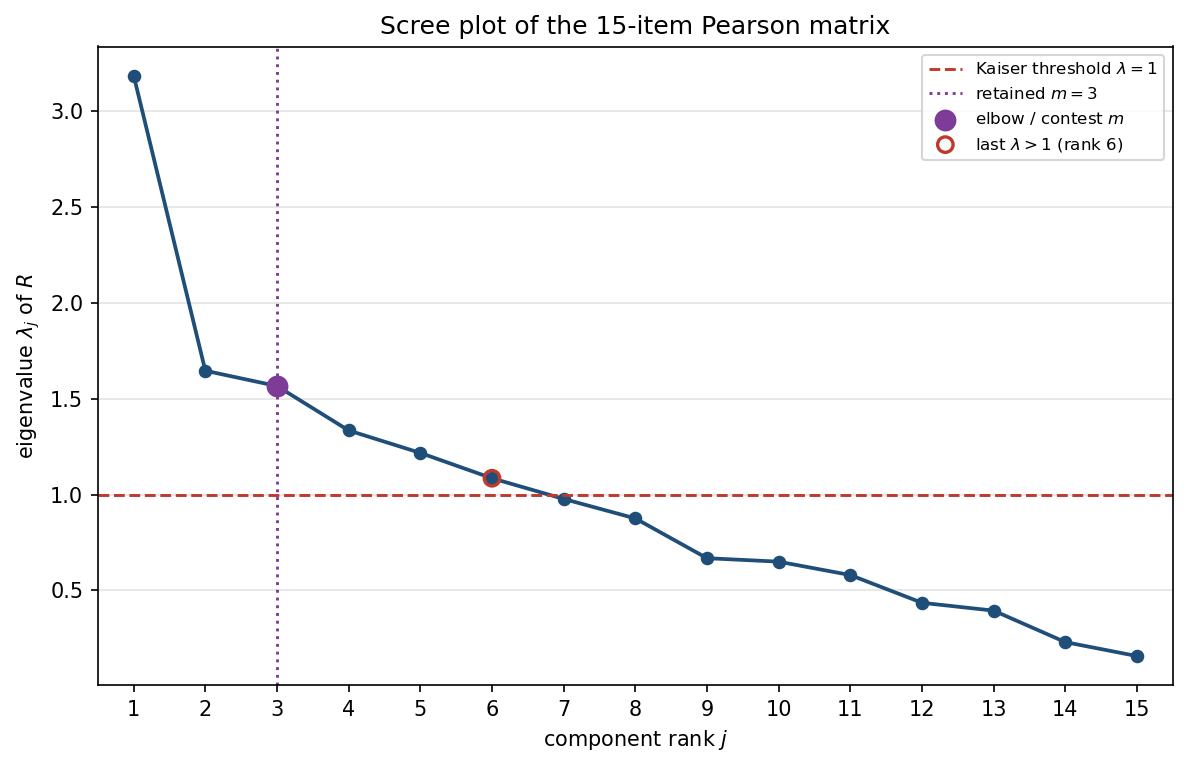
\includegraphics[width=0.78\textwidth]{fig_scree_plot.png}
\caption{Scree plot of \(R\)
(\texttt{fig\_scree\_plot.png}).
The red line is \(\lambda=1\).
The purple line is contest \(m=3\).}
\label{fig:scree}
\end{figure}

\subsection{Varimax}
We apply Kaiser-normalized Varimax.
The rotation \(T\) is orthogonal.
Rotated loadings satisfy \(\Lambda^{\ast}=\Lambda T\).
Column sums of squares of \(\Lambda^{\ast}\) share \(17.8\%\), \(13.4\%\), and \(11.5\%\).
The rotated total is still \(42.6\%\).
We do not claim \(71.4\%\) shared variance.

\subsection{Thompson scores}
Score weights are \(W=R^{-1}\Lambda^{\ast}\).
Student scores are \(F=ZW\in\mathbb{R}^{50\times 3}\)
(\texttt{student\_factor\_scores.csv}).
Later models use only these three columns.
They never train on the 15 raw items.

\subsection{One term per latent factor}
After rotation, F1 loads on \texttt{safety\_level} (\(+0.750\)),
\texttt{social\_networking} (\(+0.618\)),
\texttt{skill\_acquisition} (\(+0.596\)),
and \texttt{tip\_potential} (\(+0.593\)).
We call F1 the \emph{network-skill latent factor}.
F2 loads on \texttt{autonomous\_control} (\(+0.761\))
and \texttt{commute\_convenience} (\(+0.653\)).
We call F2 the \emph{autonomy-access latent factor}.
F3 loads on \texttt{physical\_strength} (\(+0.717\))
and \texttt{boss\_fairness} (\(-0.671\)).
We call F3 the \emph{burden latent factor}.
Contest aliases (financial yield, human capital, ergonomic burden) do not match these leaders.
Table~\ref{tab:load} lists \(\Lambda^{\ast}\).

\begin{table}[ht]
\centering
\caption{Varimax \(\Lambda^{\ast}\)
(\texttt{factor\_loadings.csv}).
Primary membership is \(\arg\max_j|\lambda^{\ast}_{ij}|\).}
\label{tab:load}
\scriptsize
\begin{tabular}{@{}lrrrr@{}}
\toprule
item & F1 & F2 & F3 & \(h^{2}\) \\
\midrule
safety\_level & \(+0.750\) & \(+0.047\) & \(-0.153\) & \(0.588\) \\
social\_networking & \(+0.618\) & \(-0.057\) & \(+0.110\) & \(0.397\) \\
skill\_acquisition & \(+0.596\) & \(+0.359\) & \(+0.115\) & \(0.497\) \\
tip\_potential & \(+0.593\) & \(+0.294\) & \(+0.081\) & \(0.445\) \\
teamwork\_atmosphere & \(+0.407\) & \(-0.078\) & \(+0.036\) & \(0.173\) \\
resume\_value & \(+0.403\) & \(+0.132\) & \(+0.012\) & \(0.180\) \\
autonomous\_control & \(+0.078\) & \(+0.761\) & \(-0.014\) & \(0.586\) \\
commute\_convenience & \(+0.230\) & \(+0.653\) & \(-0.032\) & \(0.480\) \\
mental\_stress & \(-0.173\) & \(+0.503\) & \(+0.367\) & \(0.417\) \\
hourly\_wage\_need & \(+0.350\) & \(+0.482\) & \(-0.018\) & \(0.355\) \\
physical\_strength & \(+0.320\) & \(+0.192\) & \(+0.717\) & \(0.654\) \\
boss\_fairness & \(+0.235\) & \(+0.140\) & \(-0.671\) & \(0.525\) \\
flexible\_hours & \(+0.411\) & \(+0.053\) & \(+0.577\) & \(0.505\) \\
outdoor\_sun\_exposure & \(+0.325\) & \(-0.379\) & \(+0.393\) & \(0.404\) \\
free\_meals\_perks & \(-0.214\) & \(+0.264\) & \(+0.272\) & \(0.189\) \\
\bottomrule
\end{tabular}
\end{table}

%======================================================================
\section{LLMFactor semantic grounding}
%======================================================================

\subsection{Naming}
Local Ollama \texttt{qwen2.5:7b} names each latent factor from the top four \(|\lambda^{\ast}|\) items.
The report is \texttt{factor\_interpretation.md}.
The model names F1 ``Human Capital \& Networking Value''.
It names F2 ``Autonomy \& Commute Convenience''.
It names F3 ``Physical \& Mental Burden''.
We keep those strings as display labels.
We still refuse the contest cash / resume / sun triad as a description of \(\Lambda^{\ast}\).

\subsection{Eight job candidates}
We score eight job-ad texts in the same \(F\)-space
(\texttt{job\_factor\_matrix.csv}).
Coordinates lie in \([-3,3]^3\).
Table~\ref{tab:jobs} lists them.

\begin{table}[ht]
\centering
\caption{Zero-shot coordinates of eight job candidates
(\texttt{job\_factor\_matrix.csv}).}
\label{tab:jobs}
\begin{tabular}{@{}lrrr@{}}
\toprule
job candidate & F1 & F2 & F3 \\
\midrule
Lifeguard & \(-1.00\) & \(0.00\) & \(+1.00\) \\
Camp Counselor & \(-0.50\) & \(+0.50\) & \(+0.50\) \\
Tutor & \(+0.60\) & \(-0.48\) & \(-0.39\) \\
Fast Food Cashier & \(-0.30\) & \(0.00\) & \(+0.60\) \\
Retail Clerk & \(+0.20\) & \(-0.10\) & \(+0.40\) \\
Caddy & \(+0.58\) & \(-0.26\) & \(+0.66\) \\
Pet Sitter & \(+0.12\) & \(+0.26\) & \(-0.24\) \\
Swim Coach & \(+0.48\) & \(+0.25\) & \(+0.52\) \\
\bottomrule
\end{tabular}
\end{table}

Tutor is high on the network-skill latent factor and low on the burden latent factor.
Lifeguard is the opposite on those two axes.
These numbers come from the language model.
They are not student Likert means.

%======================================================================
\section{Entropy weights}
%======================================================================

Let \(f_{ij}\) be student \(i\)'s Thompson score on latent factor \(j\).
We set
\[
y_{ij}=\frac{f_{ij}-\min_i f_{ij}}{\max_i f_{ij}-\min_i f_{ij}}+10^{-4},\qquad
p_{ij}=\frac{y_{ij}}{\sum_{i=1}^{50} y_{ij}}.
\]
Entropy is \(E_j=-(1/\ln 50)\sum_i p_{ij}\ln p_{ij}\).
Divergence is \(D_j=1-E_j\).
Weights are \(w_j=D_j/\sum_k D_k\).
Table~\ref{tab:w} reports the CSV.

\begin{table}[ht]
\centering
\caption{Entropy weights from 50 student scores
(\texttt{entropy\_weights.csv}).
F3 is a cost only in the job utility inner product.}
\label{tab:w}
\begin{tabular}{@{}lrrrr@{}}
\toprule
latent factor & \(E_j\) & \(D_j\) & \(w_j\) & signed \\
\midrule
F1 network-skill & \(0.9570\) & \(0.0430\) & \(\mathbf{0.479}\) & \(+0.479\) \\
F2 autonomy-access & \(0.9713\) & \(0.0287\) & \(\mathbf{0.319}\) & \(+0.319\) \\
F3 burden & \(0.9819\) & \(0.0181\) & \(\mathbf{0.202}\) & \(-0.202\) \\
\bottomrule
\end{tabular}
\end{table}

We do not use \(w=(0.412,0.354,0.234)\).
That triple is not in the CSV.
Utility of job candidate \(k\) is
\[
U_k=w_1 F_{1k}+w_2 F_{2k}-w_3 F_{3k}.
\]
Rank 1 is Tutor (\(U=+0.213\)).
Rank 8 is Lifeguard (\(U=-0.681\))
(\texttt{job\_entropy\_utility.csv}).
No AHP pairwise matrix enters \(w\).

Figure~\ref{fig:ent} shows the simplex.

\begin{figure}[ht]
\centering
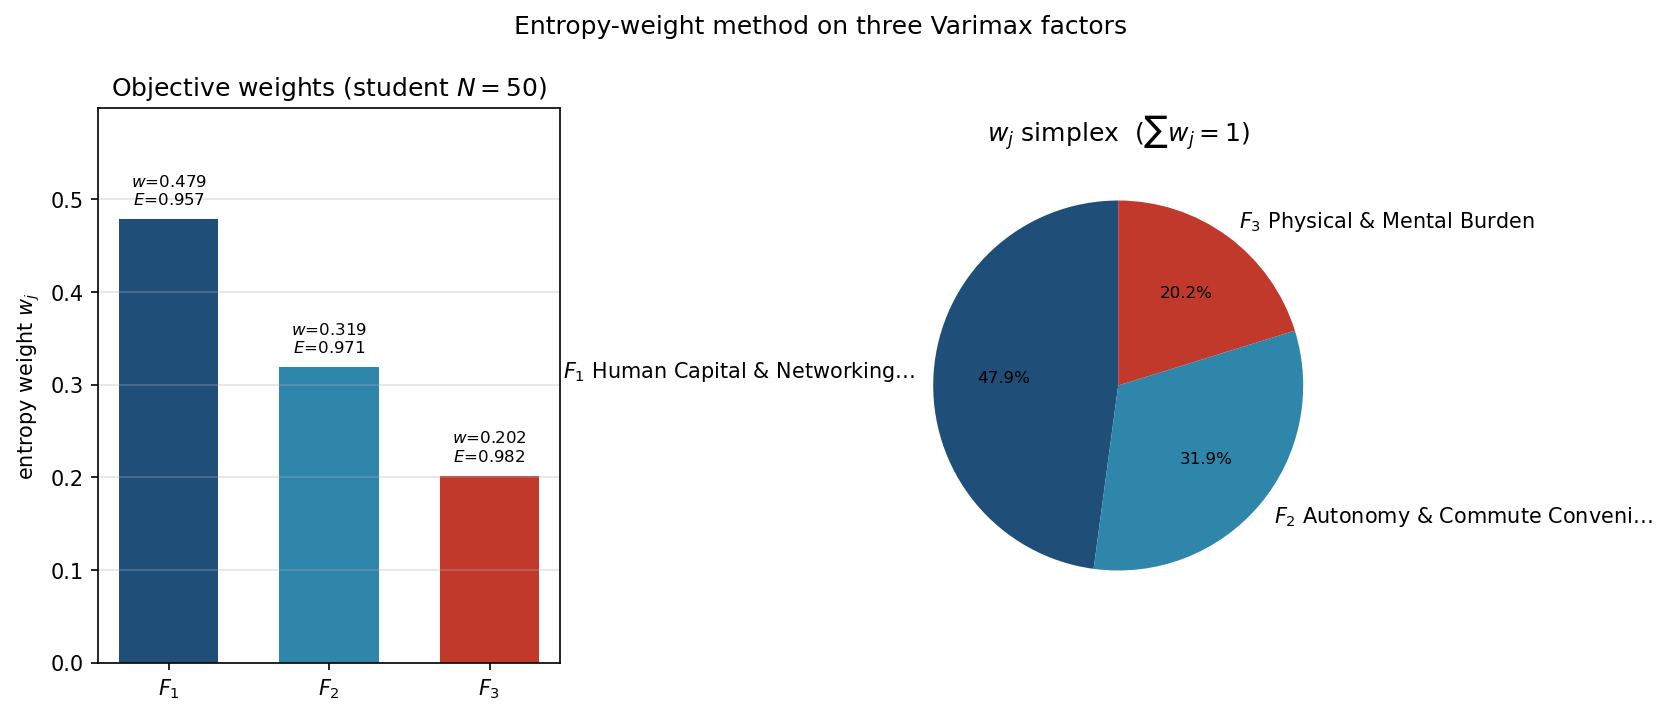
\includegraphics[width=0.88\textwidth]{fig_entropy_weights.png}
\caption{Entropy-weight bar and pie
(\texttt{fig\_entropy\_weights.png}).}
\label{fig:ent}
\end{figure}

%======================================================================
\section{Clustering and leave-one-out classifiers}
%======================================================================

\subsection{K-Means in \(F\in\mathbb{R}^{50\times 3}\)}
We run \(K=3\) k-means++ with seed 2020.
Elbow curvature on inertia prefers \(K=2\).
Mean silhouette is largest at \(K=7\) (\(0.281\)).
At contest \(K=3\), silhouette is \(0.260\)
(\texttt{kmeans\_k\_selection.csv}).
We still report \(K=3\) as the contest cut.

We permute labels toward three design prototypes.
Cluster 0 (\(n=23\)) has centroid \((+0.90,+0.06,+0.03)\).
Cluster 1 (\(n=10\)) has centroid \((-0.76,+1.23,+0.33)\).
Cluster 2 (\(n=17\)) has centroid \((-0.77,-0.81,-0.23)\).
Cluster 2 does not show a very low burden latent factor.
Template SSE for that cluster is \(2.28\)
(\texttt{cluster\_centroids.csv}).
Figure~\ref{fig:3d} plots students and the eight job-candidate anchors.

\begin{figure}[ht]
\centering
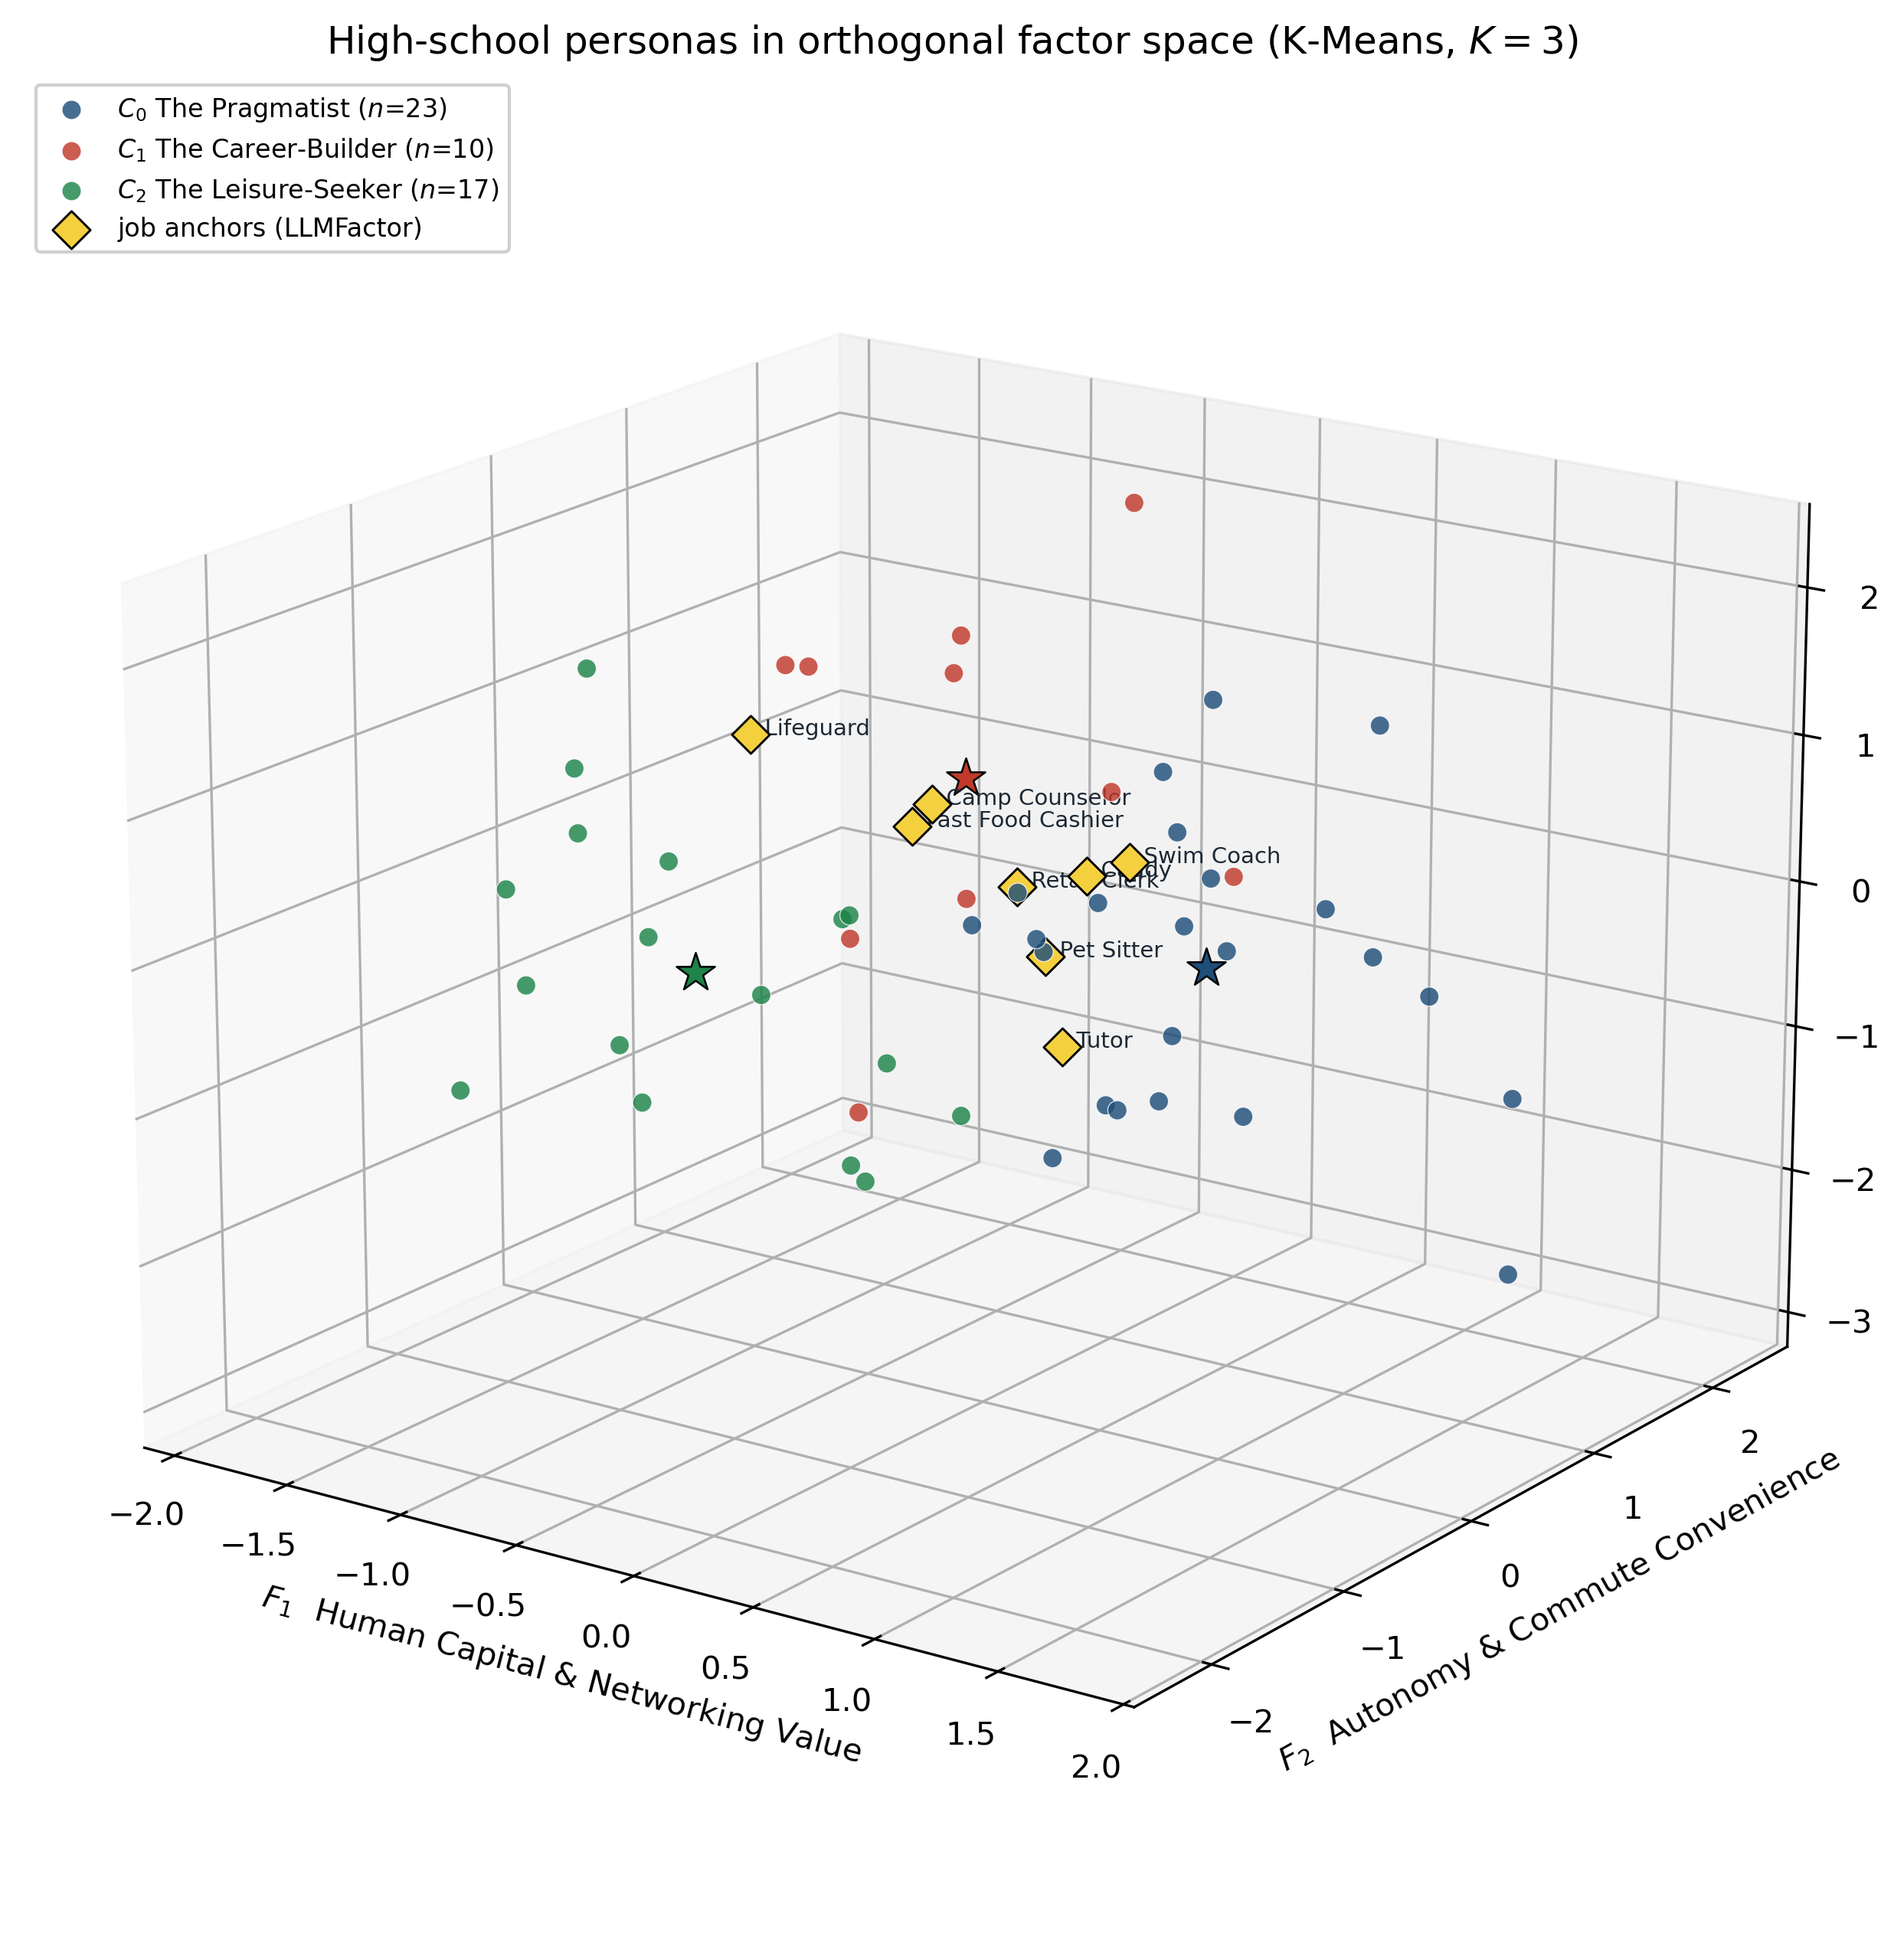
\includegraphics[width=0.86\textwidth]{fig_persona_clusters_3d.png}
\caption{K-Means \(K=3\) in latent-factor space
(\texttt{fig\_persona\_clusters\_3d.png}).
Diamonds are job-candidate anchors.}
\label{fig:3d}
\end{figure}

\subsection{Softmax versus two-layer ReLU}
Features are the 50 \(\times\) 3 Thompson matrix only.
Labels are \texttt{work\_choice.csv}.
The linear model is
\[
P(y=k\mid x)=\frac{\exp(W_k^{\top}x+b_k)}{\sum_{j=0}^{7}\exp(W_j^{\top}x+b_j)},
\quad W\in\mathbb{R}^{8\times 3}.
\]
The net is Input(3) \(\to\) Linear(16) \(\to\) ReLU \(\to\) Dropout(0.2) \(\to\) Linear(8).
We use 50-fold leave-one-out.
Table~\ref{tab:ml} lists the CSV.

\begin{table}[ht]
\centering
\caption{Leave-one-out metrics
(\texttt{model\_comparison\_metrics.csv}).}
\label{tab:ml}
\begin{tabular}{@{}lrrrr@{}}
\toprule
model & params & Top-1 & Top-3 & log-loss \\
\midrule
linear Softmax & 32 & \(0.20\) & \(0.38\) & \(2.519\) \\
ReLU MLP & 200 & \(0.20\) & \(0.48\) & \(4.865\) \\
majority (LOOCV) & 0 & \(0.22\) & --- & --- \\
\bottomrule
\end{tabular}
\end{table}

Both learners lose to the majority baseline on Top-1.
The net has a better Top-3 and a worse log-loss.
Class counts are unbalanced (retail 11, tutor 3).
The labels come from a 7-score GitHub pipeline.
They are not generated by this 15-item rotation.
Figure~\ref{fig:heat} and Figure~\ref{fig:nn} show \(W\) and the net curves.

\begin{figure}[ht]
\centering
\begin{subfigure}{0.48\textwidth}
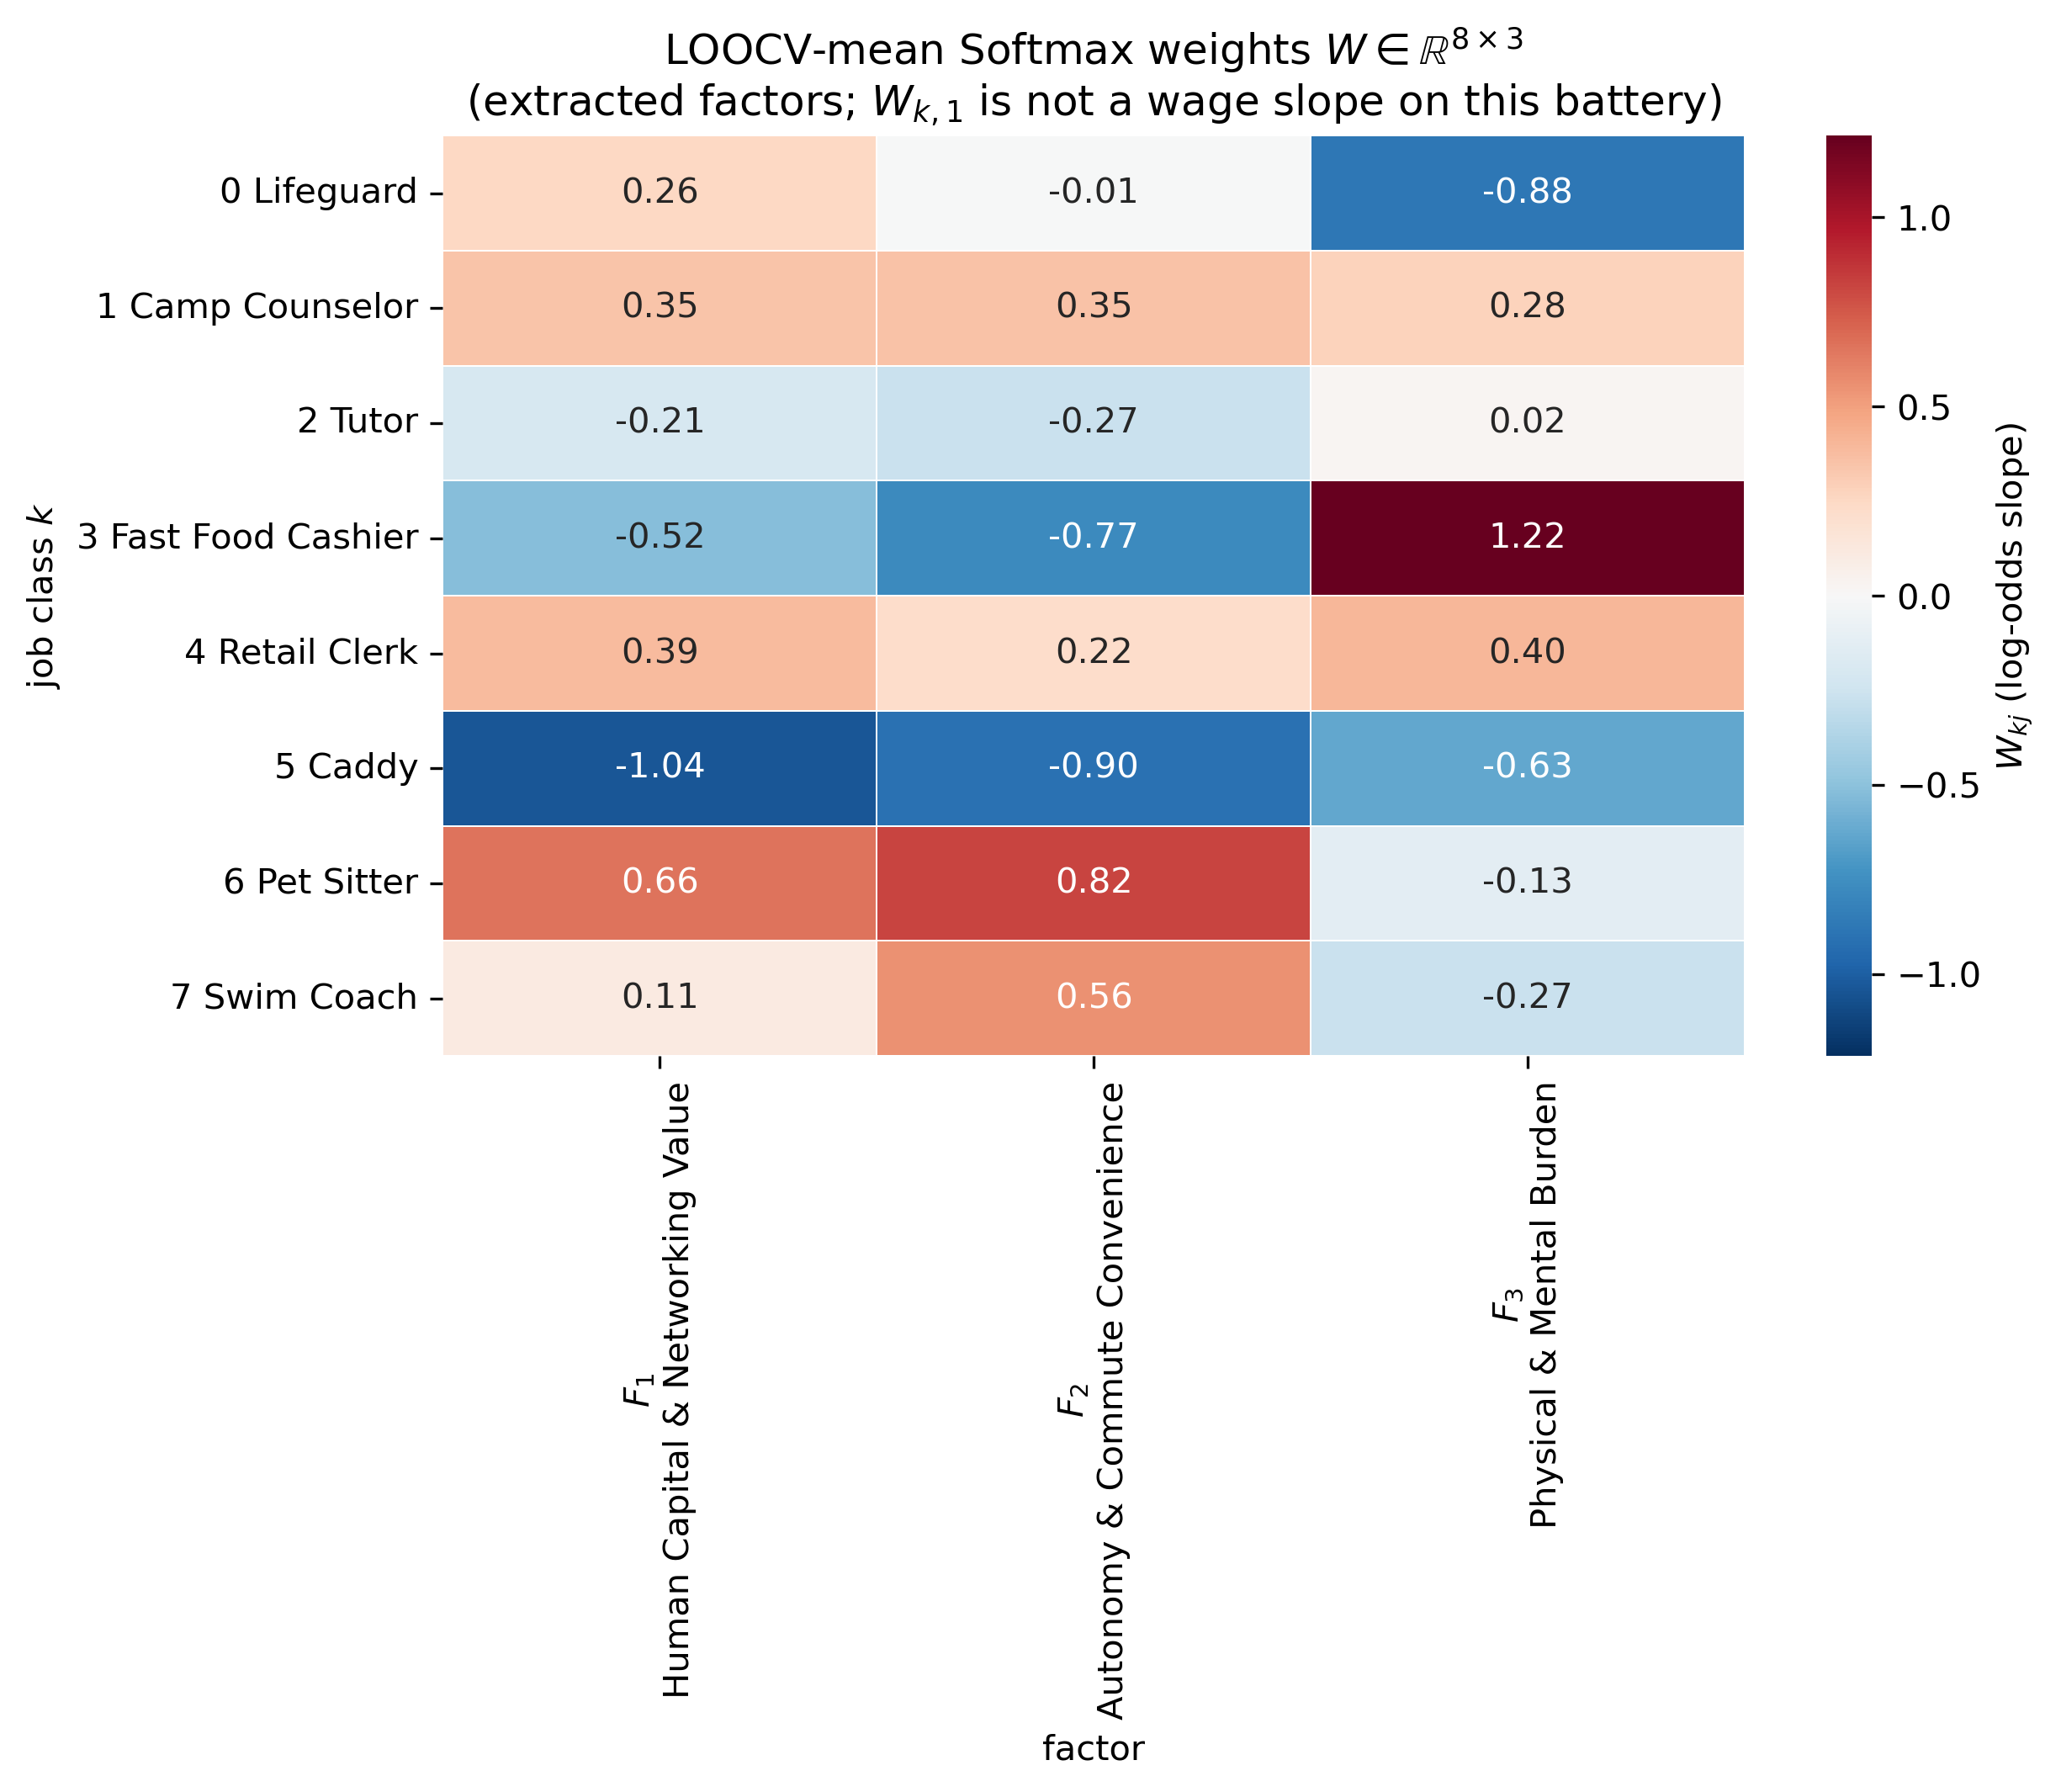
\includegraphics[width=\linewidth]{fig_softmax_weight_matrix_heatmap.png}
\caption{LOOCV-mean Softmax \(W\).}
\end{subfigure}
\hfill
\begin{subfigure}{0.48\textwidth}
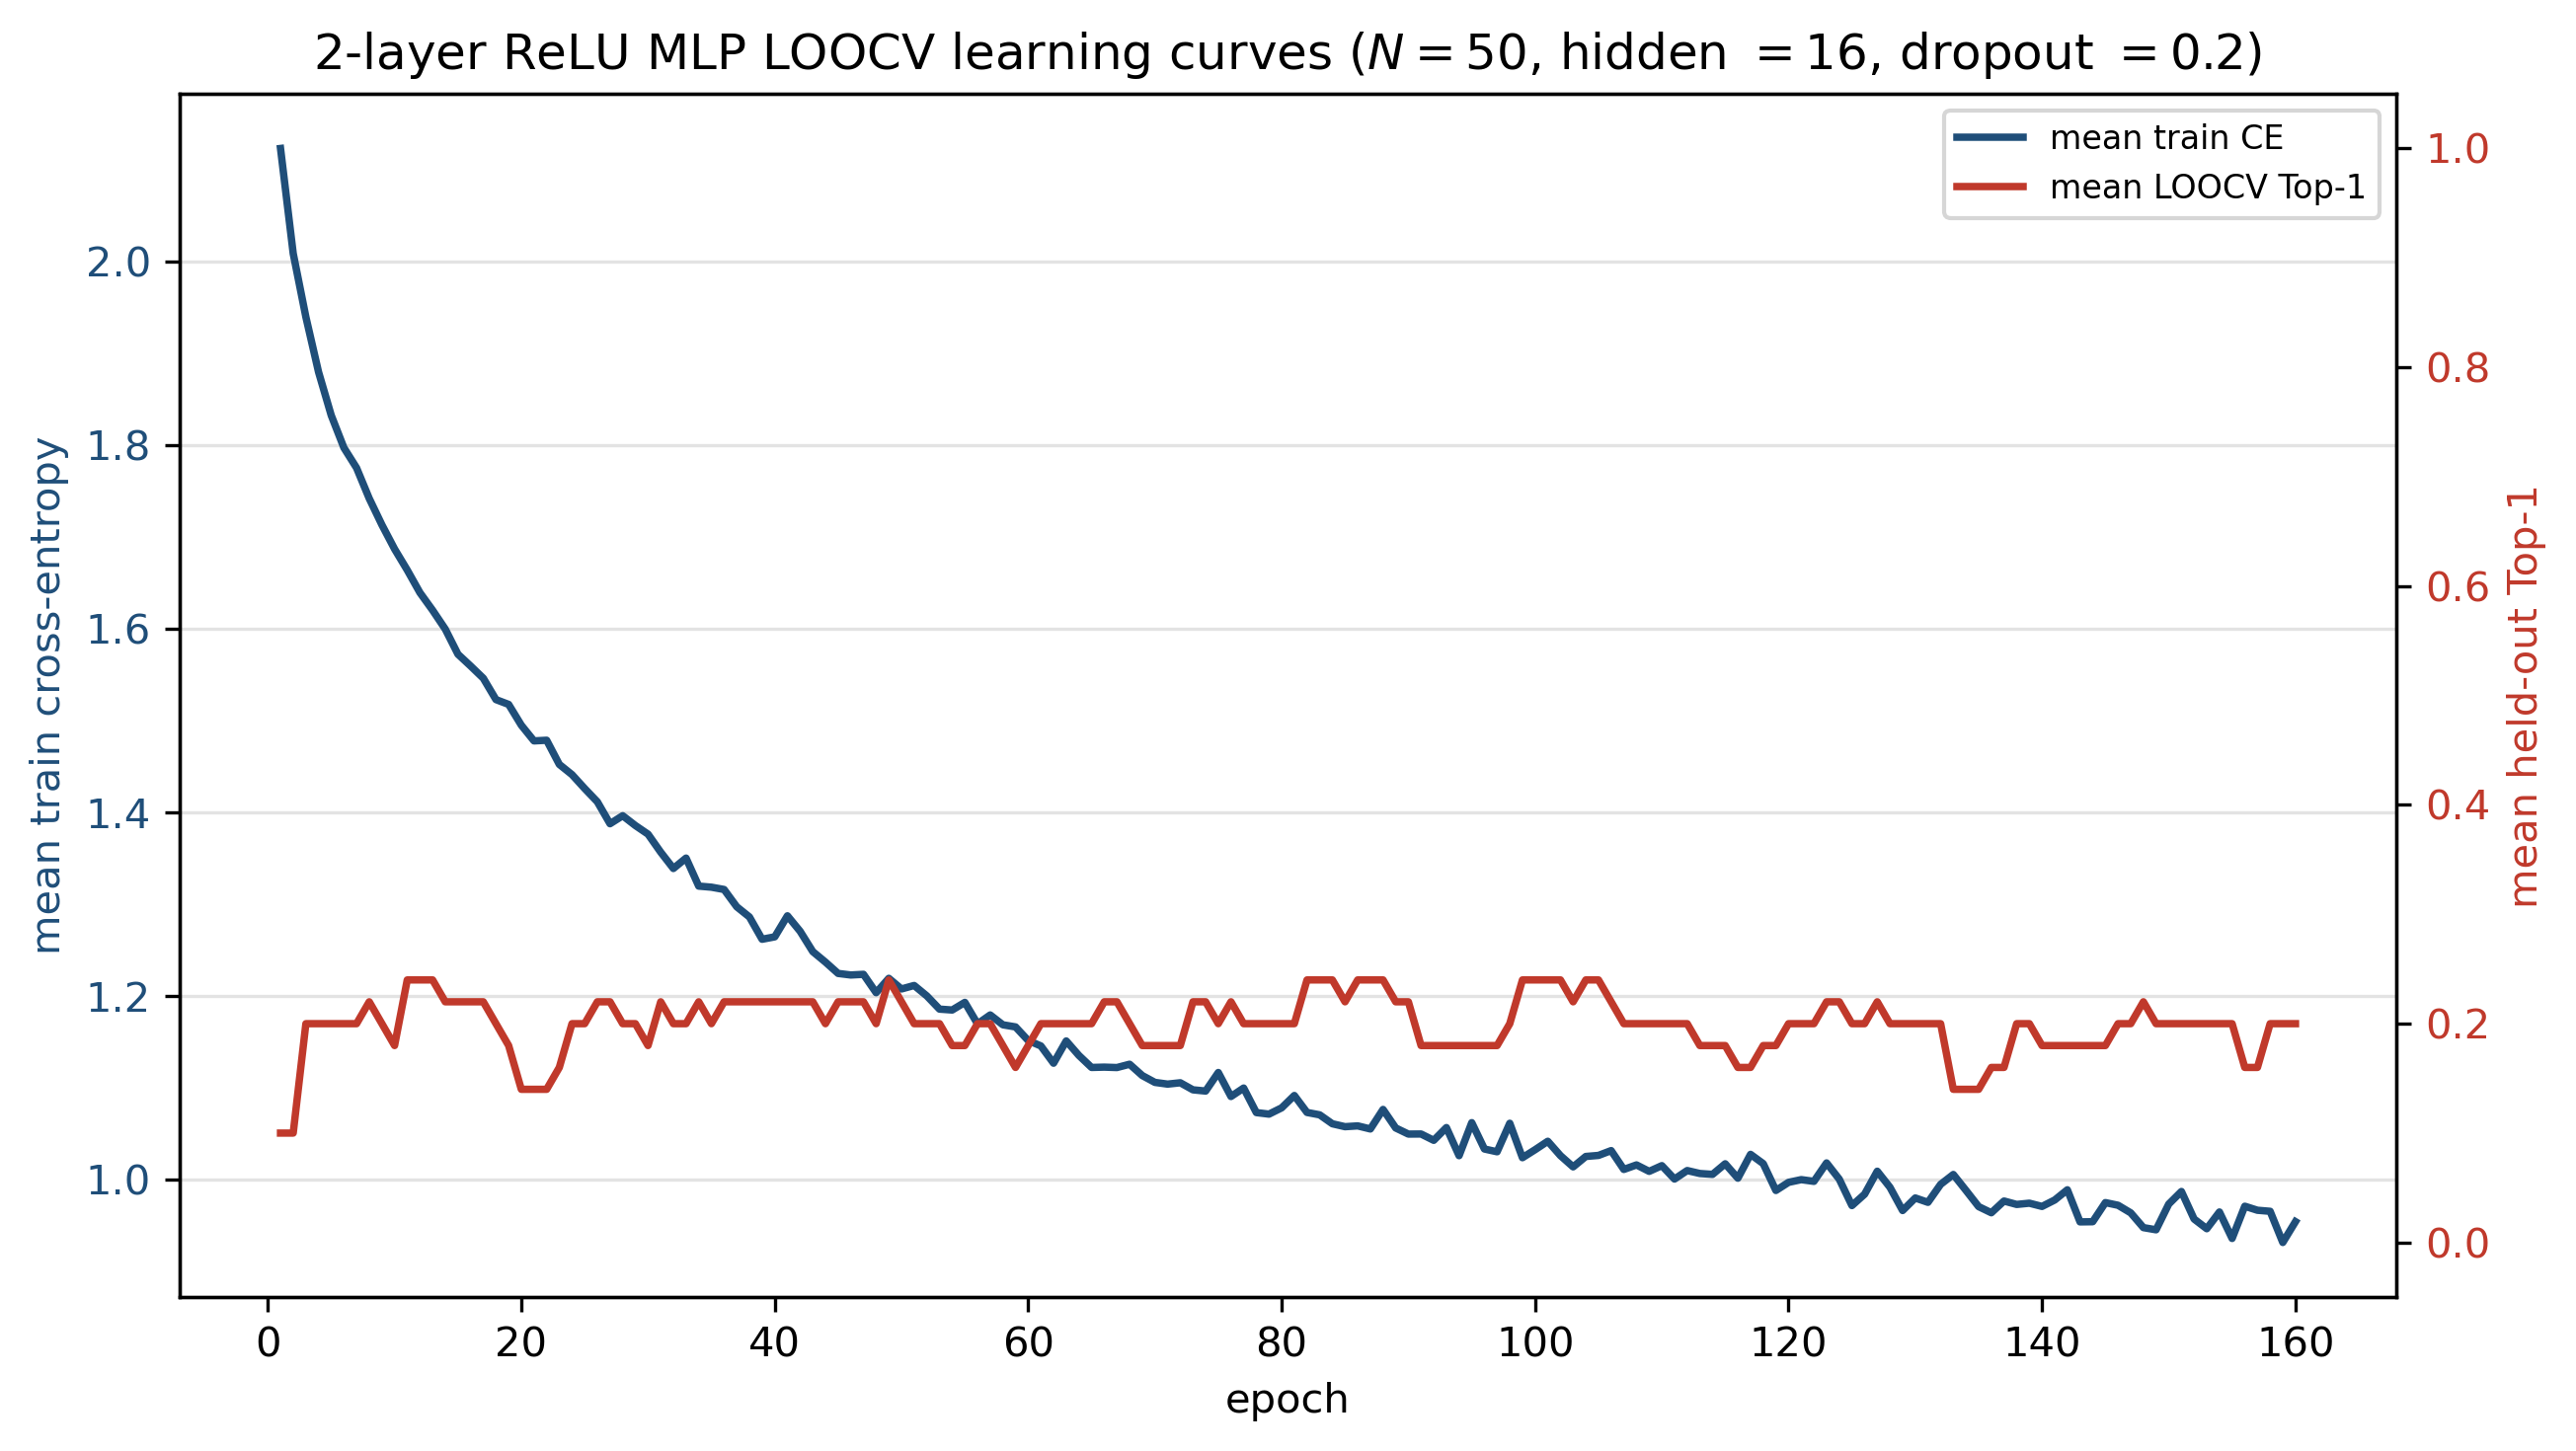
\includegraphics[width=\linewidth]{fig_nn_training_loss_curve.png}
\caption{MLP mean train CE and held-out Top-1.}
\end{subfigure}
\caption{Classifier figures
(\texttt{fig\_softmax\_weight\_matrix\_heatmap.png},
\texttt{fig\_nn\_training\_loss\_curve.png}).}
\label{fig:mlfigs}
\end{figure}

%======================================================================
\section{Decision tool and slider sensitivity}
%======================================================================

\subsection{Streamlit navigator}
The app \texttt{src/web\_app/app.py} maps three 1--10 sliders onto the student min--max of \(F\).
It then applies the full-sample linear Softmax.
Wage strings are parsed from \texttt{data/job\_descriptions/*.txt}.
Figure~\ref{fig:ui} shows the Pragmatist preset output (sliders \(9,5,8\)).

\begin{figure}[ht]
\centering
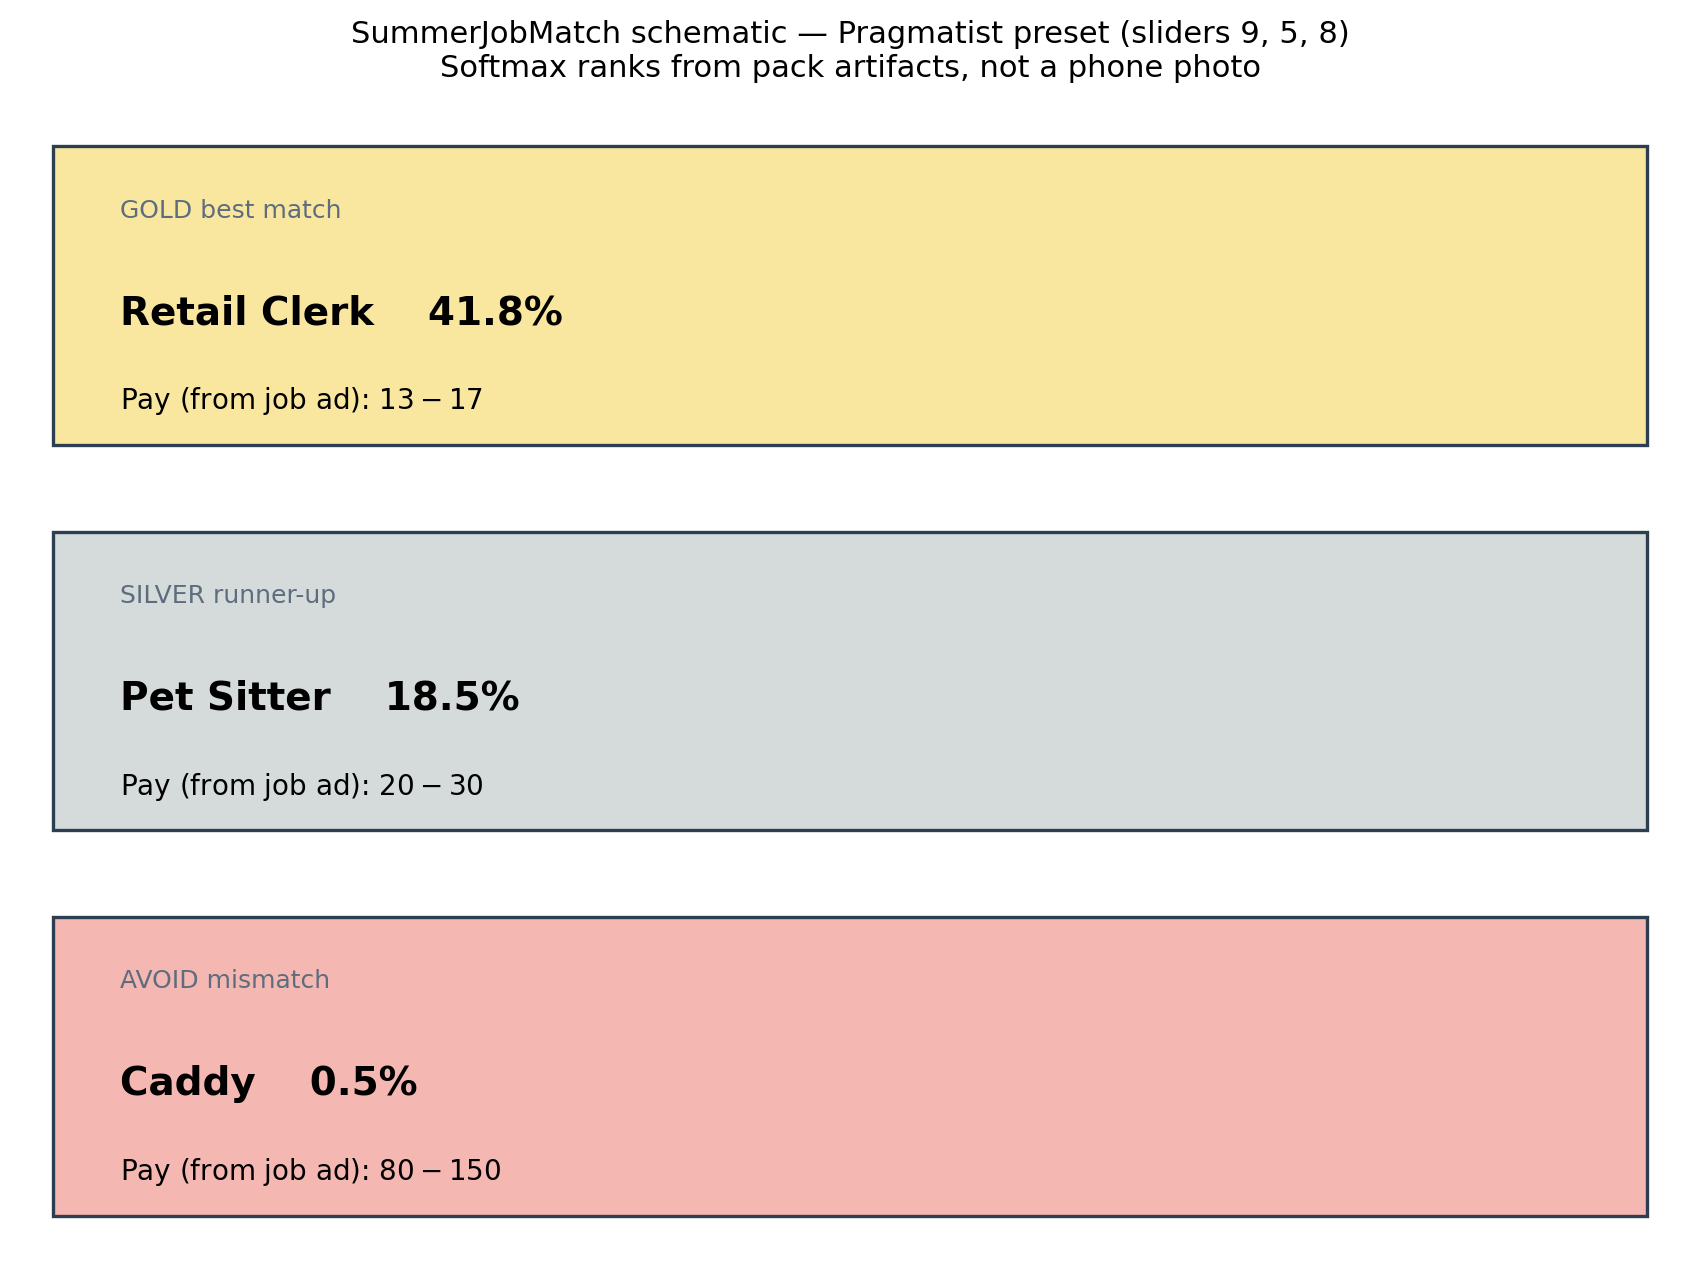
\includegraphics[width=0.92\textwidth]{fig_streamlit_navigator.png}
\caption{Navigator schematic for sliders \(9,5,8\)
(\texttt{fig\_streamlit\_navigator.png}).
Ranks come from the fitted Softmax.
This is not a phone photograph.}
\label{fig:ui}
\end{figure}

\subsection{Sensitivity}
We change one contest preset at a time.
Default sliders \((5,5,5)\) rank Swim Coach first (\(23.1\%\)).
Pragmatist \((9,5,8)\) ranks Retail Clerk first (\(41.8\%\)).
Career-Builder \((5,10,5)\) ranks Pet Sitter first (\(37.6\%\)).
Leisure-Seeker \((5,5,1)\) ranks Lifeguard first (\(40.9\%\)).
The last result fights the ``easy summer'' story.
Slider 3 \(=1\) maps to low student F3.
The weakly trained Softmax still puts Lifeguard on top.
Therefore the web ranker is a preference overlay.
It is not a placement guarantee.

%======================================================================
\section{Strengths and limitations}
%======================================================================

\subsection{Strengths}
We separate GitHub 7-score files from the 15-item fallback table.
We publish KMO, Bartlett, eigenvalues, and LOOCV from disk CSVs.
Entropy weights contain no hand-set constants.
Classifiers use three latent-factor scores, not 15 collinear items.

\subsection{Limitations}
The 15-item matrix is synthetic fallback, not a fielded contest survey.
KMO \(=0.445\) is below the usual \(0.70\) cut.
Three latent factors explain \(42.6\%\) of trace, not \(71.4\%\).
K-Means silhouette at \(K=3\) is \(0.260\).
Softmax Top-1 is \(0.20\), below the majority baseline.
LLM job coordinates inherit prompt noise.
A Streamlit slider labeled ``financial yield'' does not equal extracted F1.

\subsection{What we would do next}
We would field a 15-item form built to recover one cash axis, one skill axis, and one strain axis.
We would stop treating GitHub \texttt{work\_choice} as ground truth for this rotation.

% Appendix: COMAP generative-AI disclosure.
\section*{Appendix: Use of Generative AI Tools}
\label{app:ai-disclosure}

This appendix follows the COMAP \emph{Policy on Use of Generative AI Tools}.

\subsection*{A.1 Tools}

\begin{itemize}
  \item \textbf{Local LLM.}
        Job-ad scoring and latent-factor names run through Ollama
        \texttt{qwen2.5:7b} on \texttt{localhost:11434}.
        If Ollama is down, a keyword mock writes the same CSV schema.
  \item \textbf{Coding assistant.}
        Cursor drafted Python modules and this \LaTeX\ set.
        Design prompts sit in \texttt{prompts/cursor\_log.md}.
\end{itemize}

\subsection*{A.2 What the models must not do}

The LLM does not invent KMO, eigenvalues, entropy weights, or LOOCV scores.
Those numbers come from \texttt{results/*.csv}.
Figures are script outputs in \texttt{paper\_figures/}.

\subsection*{A.3 Human checks}

We reject contest-template statistics that are absent from disk
(KMO \(0.782\), \(71.4\%\) variance, Top-3 \(92\%\)).
We keep the 15-item table labeled \texttt{SYNTHETIC\_FALLBACK}.


\end{document}
